%! Author = t.kramer
%! Date = 10/06/2023

\section{Problem definition}
\label{sec:jp-iii-problem-definition}

% INTRO
Thermally comfortable indoor spaces have been associated with a positive influence on occupant health \citep{Altomonte2020}, satisfaction \citep{Frontczak2011, Wagner2007}, and work performance \citep{Wyon2013, Tanabe2015, Porras-Salazar2021}. However, the actual experience of occupants in many modern buildings is increasingly characterised by dissatisfaction and discomfort \citep{Graham2021}. 

Essentially, this problem goes back to the way we design and condition our buildings. A misconception of the 20th century was that thermal comfort is largely uniform between individuals and can therefore be estimated using aggregate models like the \gls{pmv} index \citep{Fanger1972}. However, recent studies show that thermal comfort is predominantly a nuanced problem, intricately linked to individual preferences and perception \citep{KramerFieldstudy2023, Gauthier2020}. Hence, typically applied "one-size-fits-all" conditioning strategies overlook the diversity in thermal comfort. On the contrary, they lead to tightly controlled indoor climates and a lack of personal influence and adaptive opportunities \citep{Humphreys1978, Aguilera2019}. The consequences are overconditioned buildings \citep{Park2018, Parkinson2021, Fukawa2021} with too narrow set point ranges \citep{Hoyt2015, Li2019, Arens2010} and undesirable occupant interventions to restore thermal comfort \citep{Hong2017}. 

This constitutes a performance gap between the intended positive impact of thermal comfort on building occupants and the negative experiences actually observed in the real world. This thermal comfort performance gap exposes significant flaws in conventional indoor climate design strategies and prompts us to challenge the underlying early thermal comfort modelling practices during the building design stage in the following section.


%%%%%%%%%%%%%%%%%%%%%%%%%%%%%%%%%%%%%%%%%%%%%%

\subsection{Status quo}

The early planning phase is associated with the greatest impact on a buildings IEQ performance and lifetime energy use \citep{Raji2017}. At this stage of the design process, the evaluation of thermal comfort provides essential feedback on the expected indoor environmental performance of the building and is the basis for key design decisions related to overall building design, conditioning strategies, and \gls{hvac} systems \citep{Yang2014, Attia2015}.


\begin{figure*}[h!]
    \centering
    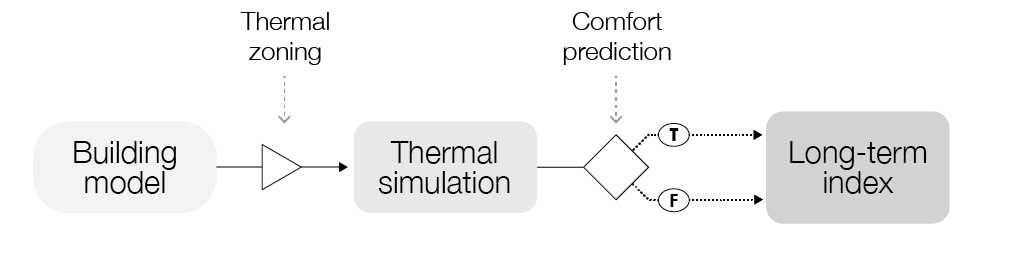
\includegraphics[width=8.9cm]{manuscript/src/figures/conventional-workflow.png}
    \caption{Simplified flow diagram of typical thermal comfort evaluation workflow: a) Simulation model is created and separated into thermal zones; b) Using thermal simulation, for each zone an annual dataset of simulated indoor climate data is generated; c) comfort model (e.g., PMV) predicts expected level of comfort; d) comfort results are summarised to long-term index (e.g., discomfort hours.) }
    \label{fig:typical-workflow}
\end{figure*}


However, despite its significant impact on operational building performance, frequent adoption in research \citep{Roetzel2012,Jafarpur2021,Silva2016, Attia2015}, and approval in international standards and certification schemes, the conventional thermal comfort evaluation workflow has several inherent limitations.


\begin{enumerate}[label={(\alph*)}]

    \item  The \textit{thermal zone} as the standard unit of analysis in \gls{bps} does not account for the spatial diversity of indoor environmental conditions in real buildings: Conventional thermal simulation engines like EnergyPlus \citep{CrawleyEnergyPlus2001} on default compute only the average indoor environmental conditions for a single node in the thermal zone centre, which corresponds to a considerable loss of potentially valuable simulation output data on spatial diversity.

    \item Aggregate thermal comfort models like the \gls{pmv} and \gls{acm} do not adequately reflect the personal variability in thermal comfort perception: Both indices show poor predictive performance when applied to individuals \citep{Cheung2019, VanHoof2008, KimZhou2018, Gauthier2020, Du2022}. Consequently, diverse occupant needs are neglected in the building design process \citep{Azar2020}.

    \item The contribution of \gls{pcs} to achieving individual thermal comfort is not considered: \gls{pcs} have been shown to significantly improve individual thermal comfort \citep{Kim2019, Knudsen2023} and to lead to a reduction in energy use by relaxing conditioning set points and reducing system capacity and \gls{hvac} operation time \citep{Rawal2020, Zhang2022}. In addition, they increase adaptive opportunities and individual control \citep{KimSchiavon2018} and promote thermal alliesthesia \citep{He2022} and satisfaction with the thermal environment \citep{Zhang2018, Kim2019}.

    \item Current comfort indices and performance metrics are overly simplified, resulting in both discomfort and excessive energy use: During the design phase, long-term thermal comfort indices play an important role in evaluating the anticipated comfort-related performance of buildings. However, it has been found that common metrics have a weak correlation with actual thermal satisfaction \citep{Li2020}, lack the necessary detail to adequately inform building design \citep{Carlucci2012}, and mainly rely on Fanger's \gls{pmv}/PPD concept \citep{Carlucci2012}, which is considered to be inadequate for long-term thermal comfort evaluation \citep{Humphreys2002, Cheung2019, Carlucci2012, Li2020}. Additionally, conventional metrics are thought to encourage active conditioning systems and energy use by leading to overly narrow temperature categories \citep{Arens2010, Hoyt2015}, and insufficiently rewarding thermal comfort achieved through passive design solutions \citep{Nicol2009}.

\end{enumerate}


Addressing these limitations can lead to an improvement of both the occupant experience and the energy efficiency in buildings. Here, the current development towards personalised thermal comfort solutions \citep{KimSchiavon2018} and an advancing digitalisation in the built environment \citep{Whyte2017} provide new opportunities to investigate and rethink conventional thermal comfort modelling practices.


%%%%%%%%%%%%%%%%%%%%%%%%%%%%%%%%%%%%%%%%%%%%%%

\subsection{Opportunities}

The recent trend of personalised comfort solutions such as \gls{pcm} and \gls{pcs} has initiated a conscious withdrawal from the common "one-size-fits-all" approach \citep{KimSchiavon2018, Rawal2020, Xie2020}. Research has shown that perception of thermal comfort is highly diverse \citep{Wang2018} and that indoor environments must provide room for adaptation and individual control \citep{VanHoof2008, Brager2015}. However, this personalisation of thermal comfort is only possible because of three particular technological developments in recent years. These can be seen as the three pillars of personal thermal comfort modelling and include advances in (a) affordable monitoring technology, (b) data science and \gls{ai} and (c) computational hardware.

The widespread adoption of cost-effective sensors for indoor environmental quality monitoring has enabled the generation of increasingly detailed datasets \citep{Chojer2020, Parkinson2019a, Li2020, Fierro2019, Kent2023}, which presents an opportunity to enhance and validate future thermal comfort simulation and prediction models. Furthermore, the combination of versatile and open-source data science software packages and potent algorithms based on \gls{ai} has enabled the transition from aggregate to personalised prediction. Together with the growing capabilities of computational hardware, especially new options provided by cloud computing \citep{Clarke2015}, these developments are set to drive innovation in thermal comfort modelling \citep{Ngarambe2020}. Taking advantage of these opportunities, comfort-related building design should aim for highly flexible spaces that facilitate individual adaptation through less energy-intensive and personalised comfort solutions (see \Cref{fig:energy-v-flexibility}).


\begin{figure*}[h!]
    \centering
    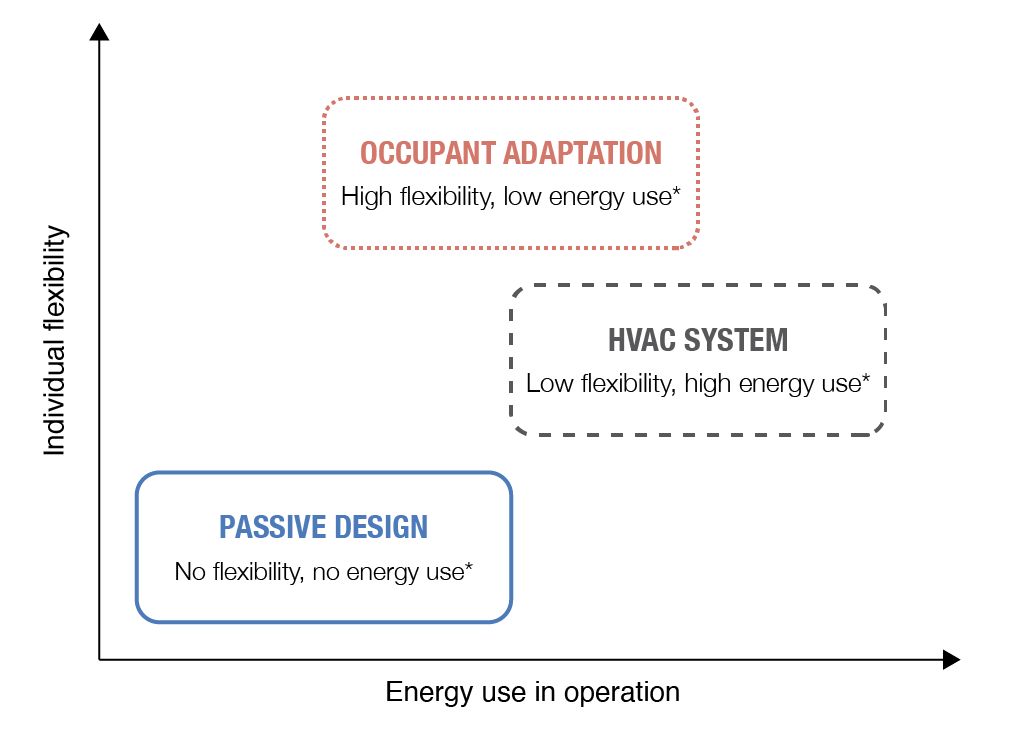
\includegraphics[width=8.9cm]{manuscript/src/figures/energy-v-flexibility.png}
    \caption{The typical tiers of a building design strategy and a comparison of their energy use and flexibility in operation: Providing opportunities for active occupant adaptation, for example, via \gls{pcs}, is the ideal complement to a passive building design, as it can at least partially replace the less flexible and energy-intensive \gls{hvac} tier, while optimising personal thermal comfort.}
    \label{fig:energy-v-flexibility}
\end{figure*}
